\chapter{Experiments}
All experiments have been conducted with some of the parameters being consistent in all the experiments. These include all convolutional layers of the residual blocks having a channel number of $256$ and a stride of $1$. The networks all have a learning rate of $0.05$, and 50 games have been played between training, and training is done with 10 training iterations between game-playing. All decisions during game play have been found through 200 MCTS simulations, with the neural network providing evaluation and guiding the search. Furthermore, all experiments have run until 1,200 training iterations have been reached, thus 6,000 games of self-play has been generated for each experiment.

Some variations have been made to measure the effect of parameter tweaking. I have created 4 main categories of experiments: (A) is the one that models AlphaZero the most, by using the original residual block design, \textit{utility} of the game result as value training target, and only asking the network in the \textit{evaluate} function in tree search; (B) is similar to A, except it uses \textit{utility} function for terminal states in \textit{evaluate}; (C) further extends B by using the found mean value of game states, during tree search, as value training targets; and finally, (D) extends C by using the full pre-activation design for its residual blocks.

\section{7x7 board}
The 1st generation of experiments I did on 7x7 boards all used half-precision both during training and self-play. All of them also used 19 residual blocks. The experiments have been labelled with a 1 appended to their corresponding category. This is listed in table \ref{table-7}.

\begin{table}[ht]
\small
\centering
\begin{tabular}{ c|| C{0.9cm}C{0.9cm}|C{0.9cm}C{0.9cm}|C{0.9cm}C{0.9cm}|C{0.9cm}C{0.9cm}C{0.9cm} }
	\hline
	Version name & \textit{A1} & \textit{A2} & \textit{B1} & \textit{B2} & \textit{C1} & \textit{C2} & \textit{D1} & \textit{D2} & \textit{D3}\\
	\hline
 	Games in storage & 500 & 1,000 & 500 & 1,000 & 500 & 1,000 & 500 & 1,000 & 1,000\\
	\hline
	Residual blocks & 19 & 13 & 19 & 13 & 19 & 13 & 19 & 13 & 19\\
	\hline
	Precision 		& half & mixed & half & mixed & half & mixed & half & mixed & mixed\\
	\hline
	Utility in evaluate & false & false & true & true & true & true & true & true & true\\
	\hline
	Value training target & utility & utility & utility & utility & mean value & mean value & mean value & mean value & mean value\\
	\hline
	Full pre-activation & false & false & false & false & false & false & true & true &true\\
	\hline 	
 	Running time & 9h 20m &  8h 19m &  7h 49m &  6h 45m &  6h 21m &  6h 16m &  8h 3m & 6h 29m & 12h 12m\\
 	\hline
\end{tabular}
\captionof{table}{List of experiments for 7x7 boards, all with 1200 training iterations and 6000 self-play games.}\label{table-7}
\end{table}

After I encountered a $\textit{NaN}$ issue while training a network in half-precision on a 9x9 board, I implemented mixed precision. Here training is done on a single precision master network, and self-play is done on a half-precision copy of the master network. All the 2nd generation experiments on 7x7 boards were done with mixed precision, and also on networks with only 13 residual blocks, but with a larger size of former games saved, 1,000 instead of only 500. Like with the 1st generations, all experiments has been labelled by category, and now with a 2 appended. A final 3rd generation experiment was also done, but only for the D category, which modelled the 2nd generation, but with 19 residual blocks. These can all be seen in table \ref{table-7}.

It should be mentioned that the running time numbers from table \ref{table-7} should be taken with a grain of salt, since the hardware the training has been performed on has not been dedicated exclusively to the experiments, i.e. other applications might have been running at the same time. Still, a tendency can be observed, that suggests: fewer residual blocks lead to faster training.

\subsection{Training losses}

\begin{figure}[ht]
	\centering
	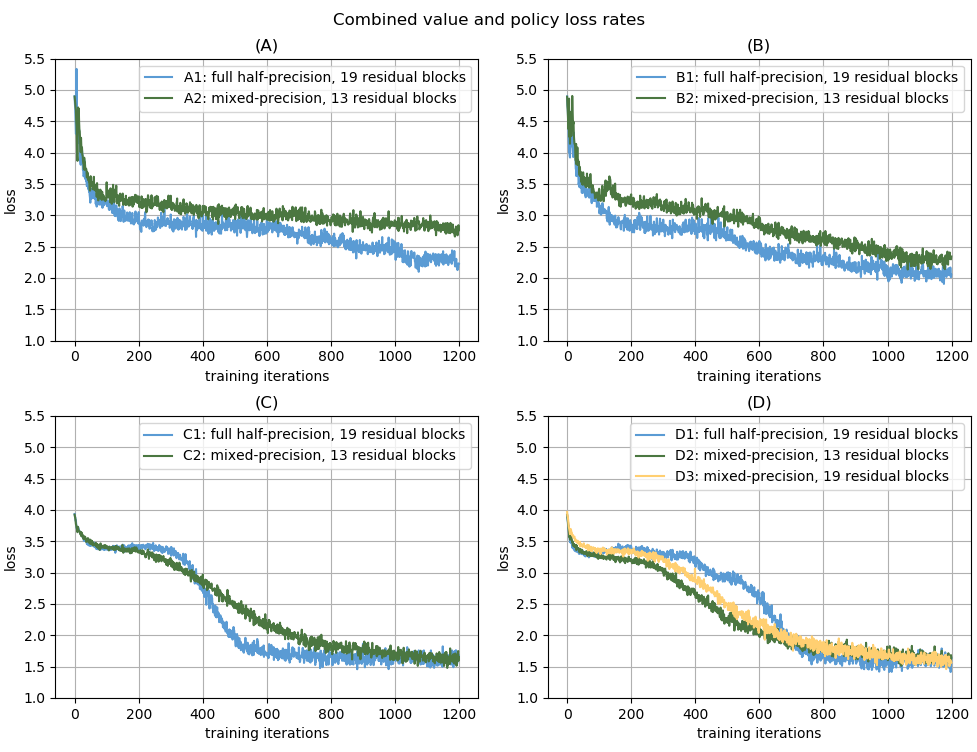
\includegraphics[width=1\textwidth]{figures/lossrates-7x7}
	\caption{Combined value and policy training loss rates for various models, trained for a 7x7 board.}
	\label{fig-loss-7}
\end{figure}

If we take a look at the combined training loss rates for the various experiments, in figure \ref{fig-loss-7}, we can see that precision type barely affects the curves. It is unfair to compare the curves of A and B, in terms of their distance to 0, with the ones from C and D, since they don't use the same value training target.

Comparing A to B, we can observe that both of the B experiments end up with a loss rate below $2.5$, whereas the shallower mixed precision experiment A2 ends above $2.5$. C and D almost have the same curves for all experiments, with the outliers being C1, which however, ends up around the same area as the others. Another interesting observation is that both of the 2nd generation experiments of A and B have curves above their 1st generation counterparts, whereas for C and D this is not the case. This indicates that either having fewer residual blocks, or having to perform single to half precision, is having a negative impact when the value training target is the utility of the game result.

\subsection{Win rates against MCTS}
Training loss rates illustrate how the neural networks perform in predicting on the training data, over time. However, they do no necessarily say anything directly about performance in playing the game. Therefore the same experiments have also been playing against the baseline MCTS agent opponent that used 2,000 simulations. For every 50 training iteration, experiments have played 20 games against this opponent, 10 as the starting player, 10 as the second player. The results can be seen in figure \ref{fig-win-7}.

\begin{figure}[ht]
	\centering
	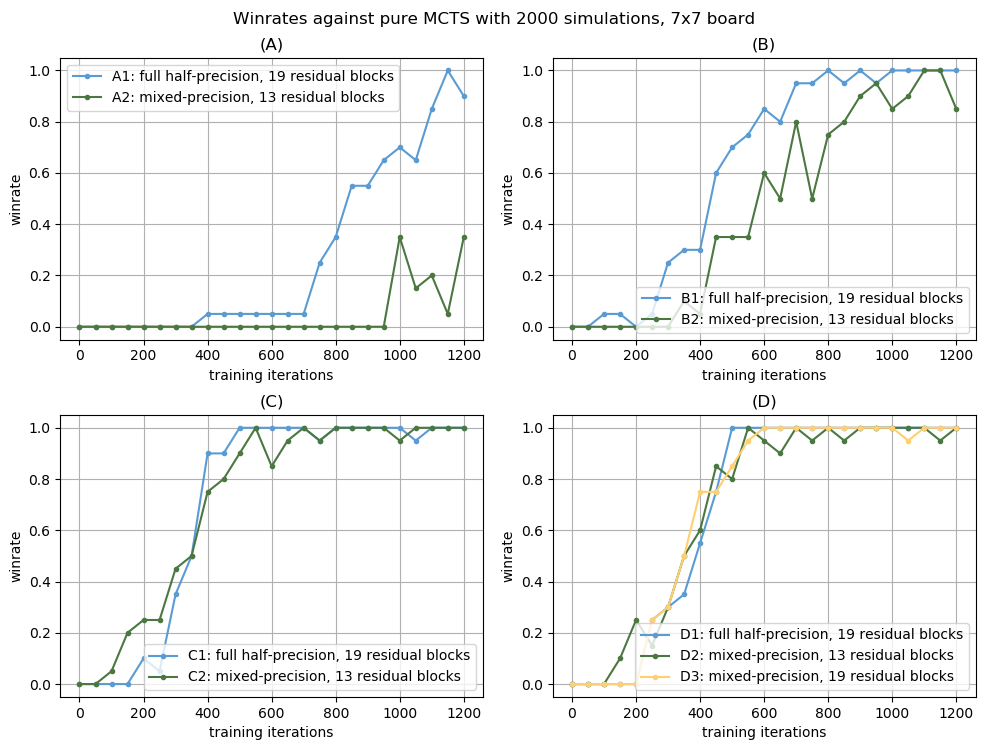
\includegraphics[width=1\textwidth]{figures/winrates-7x7}
	\caption{Winrates of various models, playing on a 7x7 board, against a purely MCTS implemented opponents, running with 2,000 simulations. Each data point is win rate from 20 games, where the learning agent model has played half as first player, and the other half as second player.}
	\label{fig-win-7}
\end{figure}

Even though the amount of games played for each data point in the lines in figure \ref{fig-win-7} are relatively few, the graphs still suggest several patterns. Both C and D, which use mean values as value training targets, reach situations where they more or less confidently beats their opponent, around 500 training iterations. Additionally for C and D, there does not seem to be much difference, whether the neural networks has 13 or 19 residual blocks, use the original residual block design or full pre-activation, or is in fully half-precision or mixed precision.

For A and B, we can observe that feeding the algorithm real game information by the utility function, for terminal states, seems to have a noticeable effect, as the B experiments reach high win rates earlier. Unlike C and D, both of the 2nd generation A and B experiments, A2 and B2, are slower at reaching the win rates of their 1st generation counter parts. Especially A2 never reaches any impressive playing performance.

The disparity of win rates between the generations of A and B interestingly coincides with the 2nd generation experiments also having higher loss rates. At the same time, for C and D, no experiments have distinct disparity in either win rates or training loss. This suggests that either the fewer residual blocks or the numerical precision conversions is harmful when using the utility value of the game result at value training target. At the same it does not seem to be harmful when using mean value as value training target.

\section{9x9 board}
For the board size of 9x9, the same experiment category definitions as for 7x7 are used, with a mapping of (E) = A, (F) = B, (G) = C, and (H) = D. For the 9x9 agent experiments, only a single generation of experiments have been done, except for H. The 2nd of H, H2, is the only agent among all experiments that has used single precision both for training and self-play. All 9x9 agents have employed neural networks 19 residual blocks deep. All 1st generation experiments have been done with mixed precision, because a failed experiment at fully half-precision resulted in all weights of the network becoming $\textit{NaN}$. A listing of the experiments can be seen in table \ref{table-9}.

\begin{table}[ht]
\small
\centering
\begin{tabular}{ c || C{0.9cm} | C{0.9cm} | C{0.9cm}| C{0.9cm} C{1.1cm}}
	\hline
	Version name & \textit{E1} & \textit{F1} & \textit{G1} & \textit{H1} & \textit{H2}\\
	\hline
 	Games in storage & 1,000 & 1,000 & 1,000 & 1,000 &1,000\\
	\hline
	Residual blocks & 19 & 19 & 19 & 19 & 19\\
	\hline
	Precision & mixed & mixed & mixed & mixed & single\\
	\hline
	Utility in evaluate & false & true & true & true & true\\
	\hline
	Value training target & utility & utility & mean value & mean value & mean value\\
	\hline
	Full pre-activation & false & false & false & true & true\\
	\hline 	
 	Running time & 21h 38m & 19h 56m & 15h 58m & 14h 41m & 1d 1h 17m \\
 	\hline
\end{tabular}
\captionof{table}{List of experiments for 9x9 boards, all with 1200 training iterations and 6000 self-play games.}\label{table-9}
\end{table}

As with the 7x7 experiments, these have been running for 1,200 training iterations, generating 6,000 self-play games. All experiments have retained the last 1,000 played games to sample training data from. Thus, even though the game complexity has been considerably increased, all the 1st generation 9x9 experiments are very similar in set-up to the 2nd generation 7x7 experiments.

Again, the running times are potentially misleading, as the hardware may have been running other processes simultaneously to the experiments. If they are to be believed, they could indicate that the G1 and H1 experiments learn more optimal plays, thus reducing the average game length, consequently reducing the required processing power to reach 6,000 self-played games. The outlier among all the 9x9 experiments is H2, which ran for more than a day.

\subsection{Training losses}
Looking at the training loss rates, in figure \ref{fig-loss-9}, once again the experiments using mean value as the value training target, G and H, are experiencing greater training losses over time. This time, however, the second drop in rates occurs later than for the C and D experiments. 

\begin{figure}[ht]
	\centering
	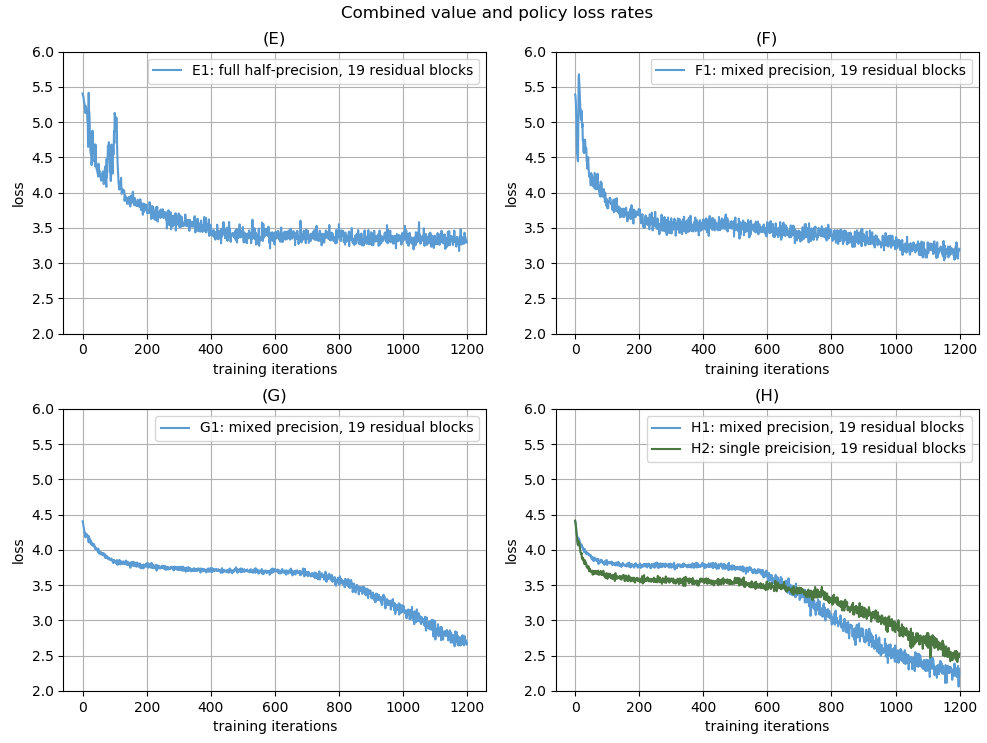
\includegraphics[width=1\textwidth]{figures/lossrates-9x9}
	\caption{Combined value and policy training loss rates for various models, trained for a 9x9 board.}
	\label{fig-loss-9}
\end{figure}

Interestingly H experiences a deeper drop than G, which also starts earlier. Among the two H experiments, H2 experiences a lower loss rate until around training iteration 700, when H1 makes a deep drop, which ends up having the lowest by the 1,200 training iteration mark. E1 and F1 follow the same slowly decreasing trend as their 7x7 mixed precision counterparts, A2 and B2.

\subsection{Win rates against MCTS}
As mentioned in chapter 2, an increase in board size from 7x7 to 9x9 greatly increases the game tree complexity. Using an MCTS opponent with only 2,000 simulations on a 9x9 board would make it significantly intellectually impaired, in contrast to when it plays on a 7x7 board. Therefore I have increased the number of simulations for the baseline MCTS agent to 10,000. However, this also increases the computation time tremendously, because the agent is not utilizing parallelism. As a consequence only 10 games have been played between the baseline MCTS and each experiment, at 50 training iterations interval, with 5 as first and 5 as second player. The resulting win rates are found in figure \ref{fig-win-9}.

\begin{figure}[ht]
	\centering
	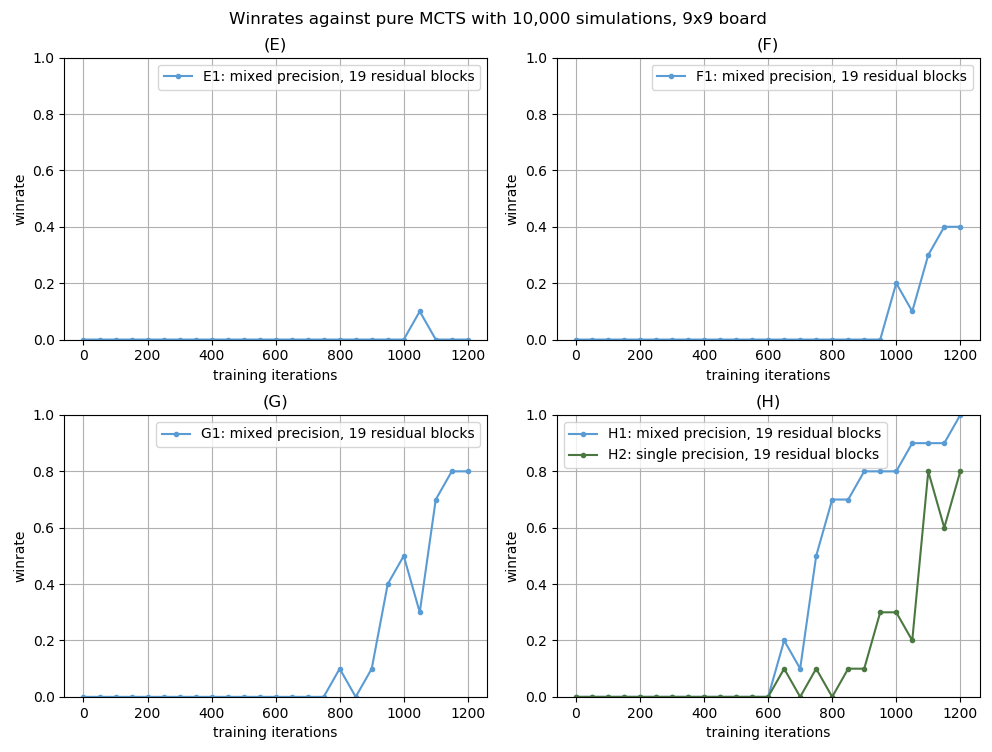
\includegraphics[width=1\textwidth]{figures/winrates-9x9}
	\caption{Win rates of various models, playing on a 9x9 board, against the baseline MCTS implemented opponent, running with 10,000 simulations. Each data point is win rate from 10 games, where the learning agent model has played half as first player, and the other half as second player.}
	\label{fig-win-9}
\end{figure}

Like with the 7x7 experiments, win rate follows training loss to a large degree, with the experiments that experienced the largest drops, also being the ones that play better. Different from 7x7, full pre-activation actually seems to perform better than the original residual block design, in that H1 has a better win rate than G1. Surprisingly E1 loses all its games, except for a single one. F1 shows almost the same low level of playing ability, but does have an up-going curve towards the end of the experiment. A final interesting observation is that the single precision version of H, H2, fares significantly worse than its mixed precision counterpart.

\subsection{Performance against Hexy}
In order to test the game playing performance against an established well-performing agent, I have conducted tests against Hexy, the agent mentioned in chapter 2. The games have been played in a round-robin tournament format\footnote{Also known as a all-play-all tournament.}. Here H1, H2, the baseline MCTS, and Hexy have all played against each other. Hexy on expert settings, and baseline MCTS with 10,000 simulations. To track the learning curve of H1 and H2, versions from 200 training iteration intervals are included. All match-ups have had the agents alternate between being first and second player, to get around the first player advantage. Furthermore, to add more certainty to the model, all H agents that have played the baseline MCTS, has done so for 10 games, 5 as first and 5 as second. All game results are listed in appendix D.

A freeware tool to estimate bayesian Elo ratings, by French computer scientist Remi Coulom, has been used to measure the playing performance of the agents\cite{Coulom}. The tool is originally created for Chess, but, to the best of my knowledge, equally suitable to the task at hand. The output of running the tool can be found in appendix C, and a graph of the results are in figure \ref{fig-elo}.

\begin{figure}[ht]
	\centering
	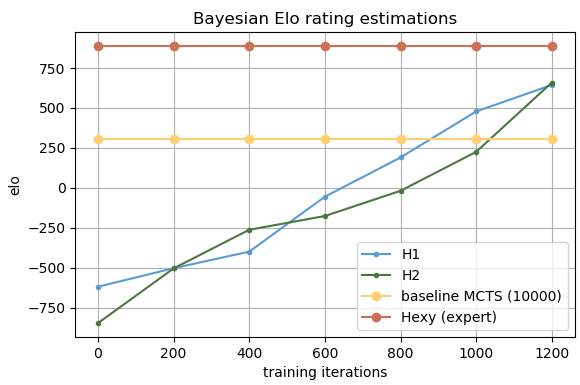
\includegraphics[width=.75\textwidth]{figures/elo}
	\caption{Bayesian Elo rating estimations for H1 and H2, over time, and static versions of Hexy on expert settings, and baseline MCTS with 10,000 simulations.}
	\label{fig-elo}
\end{figure}

For the games supporting figure \ref{fig-elo}, Hexy did not lose a single game. Interestingly, according to the estimates, H2, actually fares slightly better than H1, for the 1,200 iteration versions. To test if is actually possible to beat Hexy, on expert settings, with an agent using this project's approach, I let H2 train for an additional 1,200 iterations.

H2 with 2,400 training iterations, and 12,000 self-play games played, spent 1 day 22 hours and 10 minutes running in total. Playing it against Hexy, still on expert settings, H2 was able to beat Hexy in the game where H2 was the first player. It lost the second game, where it was the second player. Including these two games in the elo estimation, Hexy and H2 with 2,400 training iterations are estimated to be of equal Elo rank. However, with a much larger uncertainty for H2. The play history of both games can be found in appendix B. The Elo estimation tables are in appendix C.
